\section{Ιδιοανυσματική ανάλυση συστήματος}

\subsection{Υπολογισμός ιδιοτιμών συστήματος}
Για την αναγνώριση των ιδιοσυχνοτήτων και της απόσβεσης του συστήματος πραγματοποιούμε ιδιοανυσματική ανάλυση. 

\noindent Αρχικά, μετασχηματίζουμε τις αεροελαστικές εξισώσεις σε μορφή κατάστασης-χώρου (state space transformation). 

\begin{equation}
    \begin{aligned}
       \mathbf{y_1} &= \dot{\mathbf{x}}\\ 
       \mathbf{y_2} &= \mathbf{x} 
    \end{aligned} 
    \label{eq:transform}
\end{equation}

Επομένως το σύστημα γίνεται

\begin{equation}
\begin{bmatrix}
\mathbf{M} & \mathbf{0}\\
\mathbf{0} & \mathbf{I}\\
\end{bmatrix}\cdot
\dot{
    \begin{Bmatrix}
    \mathbf{y_1}\\
    \mathbf{y_2}
    \end{Bmatrix}
    } = 
    \begin{bmatrix}
        -\mathbf{C} & -\mathbf{K}\\
        \mathbf{I} & \mathbf{0}\\
    \end{bmatrix}\cdot
    \begin{Bmatrix}
    \mathbf{y_1}\\
    \mathbf{y_2}
    \end{Bmatrix}
    +
    \begin{Bmatrix}
    \mathbf{Q}\\
    \mathbf{0}
    \end{Bmatrix}
    \label{eq:statespace}
\end{equation}

Και εναλλακτικά

\begin{equation}
\dot{
    \begin{Bmatrix}
    \mathbf{y_1}\\
    \mathbf{y_2}
    \end{Bmatrix}
    } = 
    \underbrace{
    \begin{bmatrix}
        -\mathbf{M^{-1} C} & -\mathbf{M^{-1} K}\\
        \mathbf{I} & \mathbf{0}\\
    \end{bmatrix}
    }_{A}
    \cdot
    \begin{Bmatrix}
    \mathbf{y_1}\\
    \mathbf{y_2}
    \end{Bmatrix}
    +
    \underbrace{
    \begin{bmatrix}
        \mathbf{M}^{-1} & \mathbf{0}\\
        \mathbf{0} & \mathbf{I}\\
    \end{bmatrix}\cdot
    \begin{Bmatrix}
    \mathbf{Q}\\
    \mathbf{0}
    \end{Bmatrix}
    }_{B}
    \label{eq:finstatespace}
\end{equation}

Αναλύοντας το ομογενές σύστημα, οι ιδιοσυχνότητες και η απόσβεση δίνονται απο τις ιδιοτιμές του μητρώου \textbf{A}. Για τους δυο βαθμούς ελευθερίας του φυσικού μας προβλήματος, το μητρώο Α έχει διαστάσεις $4x4$ και συνεπώς δίνει τέσσερις ιδιοτιμές -- δύο ζεύγη μιγαδικών συζυγών ιδιοτιμών απο την λύση της \cref{eq:eigenvalues}. 

\begin{equation}
    det(\mathbf{A}-\lambda_i\mathbf{I})=0
\label{eq:eigenvalues}
\end{equation}

Σημειώνεται πως στην πράξη, για μητρώα μεγαλύτερα του $2x2$ οι ιδιοτιμές δεν βρίσκονται λύνοντας την \cref{eq:eigenvalues} αλλά βρίσκονται αριθμητικά απο το μητρώο \textbf{A}.

Κάθε ζεύγος συζυγών ιδιοτιμών πλεον έχει την παρακάτω μορφή (\cref{eq:eigenvalue}).

\begin{equation}
    \lambda_i, \lambda_i^c = -\zeta \pm i\underbrace{\omega_n\sqrt{1-\zeta^2}}_{\omega_d}
    \label{eq:eigenvalue}
\end{equation}

Επομένως, το πραγματικό μέρος της ιδιοτιμής μας πληροφορεί για την απόσβεση του συστήματος για συχνότητα ταλάντωσης $\omega_d$ και το φανταστικό μέρος μα δίνει την ιδιοσυχνότητα του συστήματος για κάθε ιδιοτιμή. 

\noindent Επιπλέον, απο την \cref{eq:eigenvectors} για κάθε ιδιοτιμή μπορούμε να βρούμε την αντίστοιχη ιδιομορφή, που μας πληροφορεί για το πλάτος της ταλάντωσης των βαθμών ελευθερίας όταν το σύστημα ταλαντώνεται με την αντίστοιχη ιδιοσυχνότητα. Στη δική μας περίπτωση  για κάθε ιδιοτιμή μπορούμε να βρούμε την αντίστοιχη ιδιομορφή, που μας πληροφορεί για τη συσχέτιση των βαθμών ελευθερίας όταν το σύστημα ταλαντώνεται με την αντίστοιχη ιδιοσυχνότητα. Κάθε ιδιομορφή συνήθως περιγράφει την κίνηση του συστήματος όπως κυριαρχείται από την ταλάντωση ενος βαθμού ελευθερίας. Σε προβλήματα περισσότερων βαθμών ελευθερίας, και ειδικά σε προβλήματα συνεχούς μέσου, υψηλότερες ιδιοτιμές περιγράφουν και πεπλεγμένες μορφές.

\begin{equation}
    (\mathbf{A}-\lambda_i\mathbf{I})\mathbf{\phi_i}=0
    \label{eq:eigenvectors}
\end{equation}

\subsection{Υπολογισμός απόσβεσης συναρτήσει της γωνίας προσβολής}

Όπως αναφέραμε και στην προηγούμενη παράγραφο, οι ιδιοτιμές του συστήματος υπολογίζονται απο το μητρώο \textbf{A} της \cref{eq:finstatespace}. Προφανώς, το μητρώο της απόσβεσης αφορά τη θέση αναφοράς γύρω απο την οποία γραμμικοποιήσαμε, και επιλέξαμε να χρησιμοποιήσουμε τις εξισώσεις μόνιμης ροής (που δεν εξαρτώνται απο την ταχύτητα ταλάντωσης) γραμμικοποιώντας γύρω απο το σημείο ισορροπίας ($\dot{u},\dot{w}=0$). 

\noindent Τα διαγράμματα μεταβολής της απόσβεσης για τους δυο βαθμούς ελευθερίας συναρτήσει της γωνίας προσβολής παρατίθενται στο σχήμα \ref{fig:damping} ενώ τα δεδομένα που χρησιμοποιήθηκαν για το μοντέλο παρατίθενται στον πίνακα \ref{tab:data}.

\begin{table}[ht!]
    \begin{center}
        \begin{tabular}[c]{|r|c|c|l|}
            \hline
            Γραμμική μάζα & $\mathbf{m}$ & 165 & $kg/m$ \\
            Ελαστικότητα $\parallel$ χορδής & $\mathbf{k_{\xi}}$ & 15791 & $N/m$ \\
            Ελαστικότητα $\perp$ χορδής & $\mathbf{k_{\zeta}}$ & 3948 & $N/m$ \\
            Ταχύτητα ελεύθερης ροής & $\mathbf{U_{inf}}$ & 80 & $m/s$ \\
            Γωνία στήριξης & $\mathbf{\theta}$ & 2 & $^o$ \\
            Γωνία προσβολής & $\mathbf{\alpha}$ & 4 & $^o$ \\
            Μήκος χορδής & $\mathbf{c}$ & 1.5 & $m$ \\
            Αριθμός Reynolds & $\mathbf{Re}$ & $8\cdot 10^6$ & -- \\
            \hline
        \end{tabular}
    \caption{Δεδομένα μοντέλου}
    \label{tab:data}
    \end{center}
\end{table}

\begin{figure}
    \begin{center}
        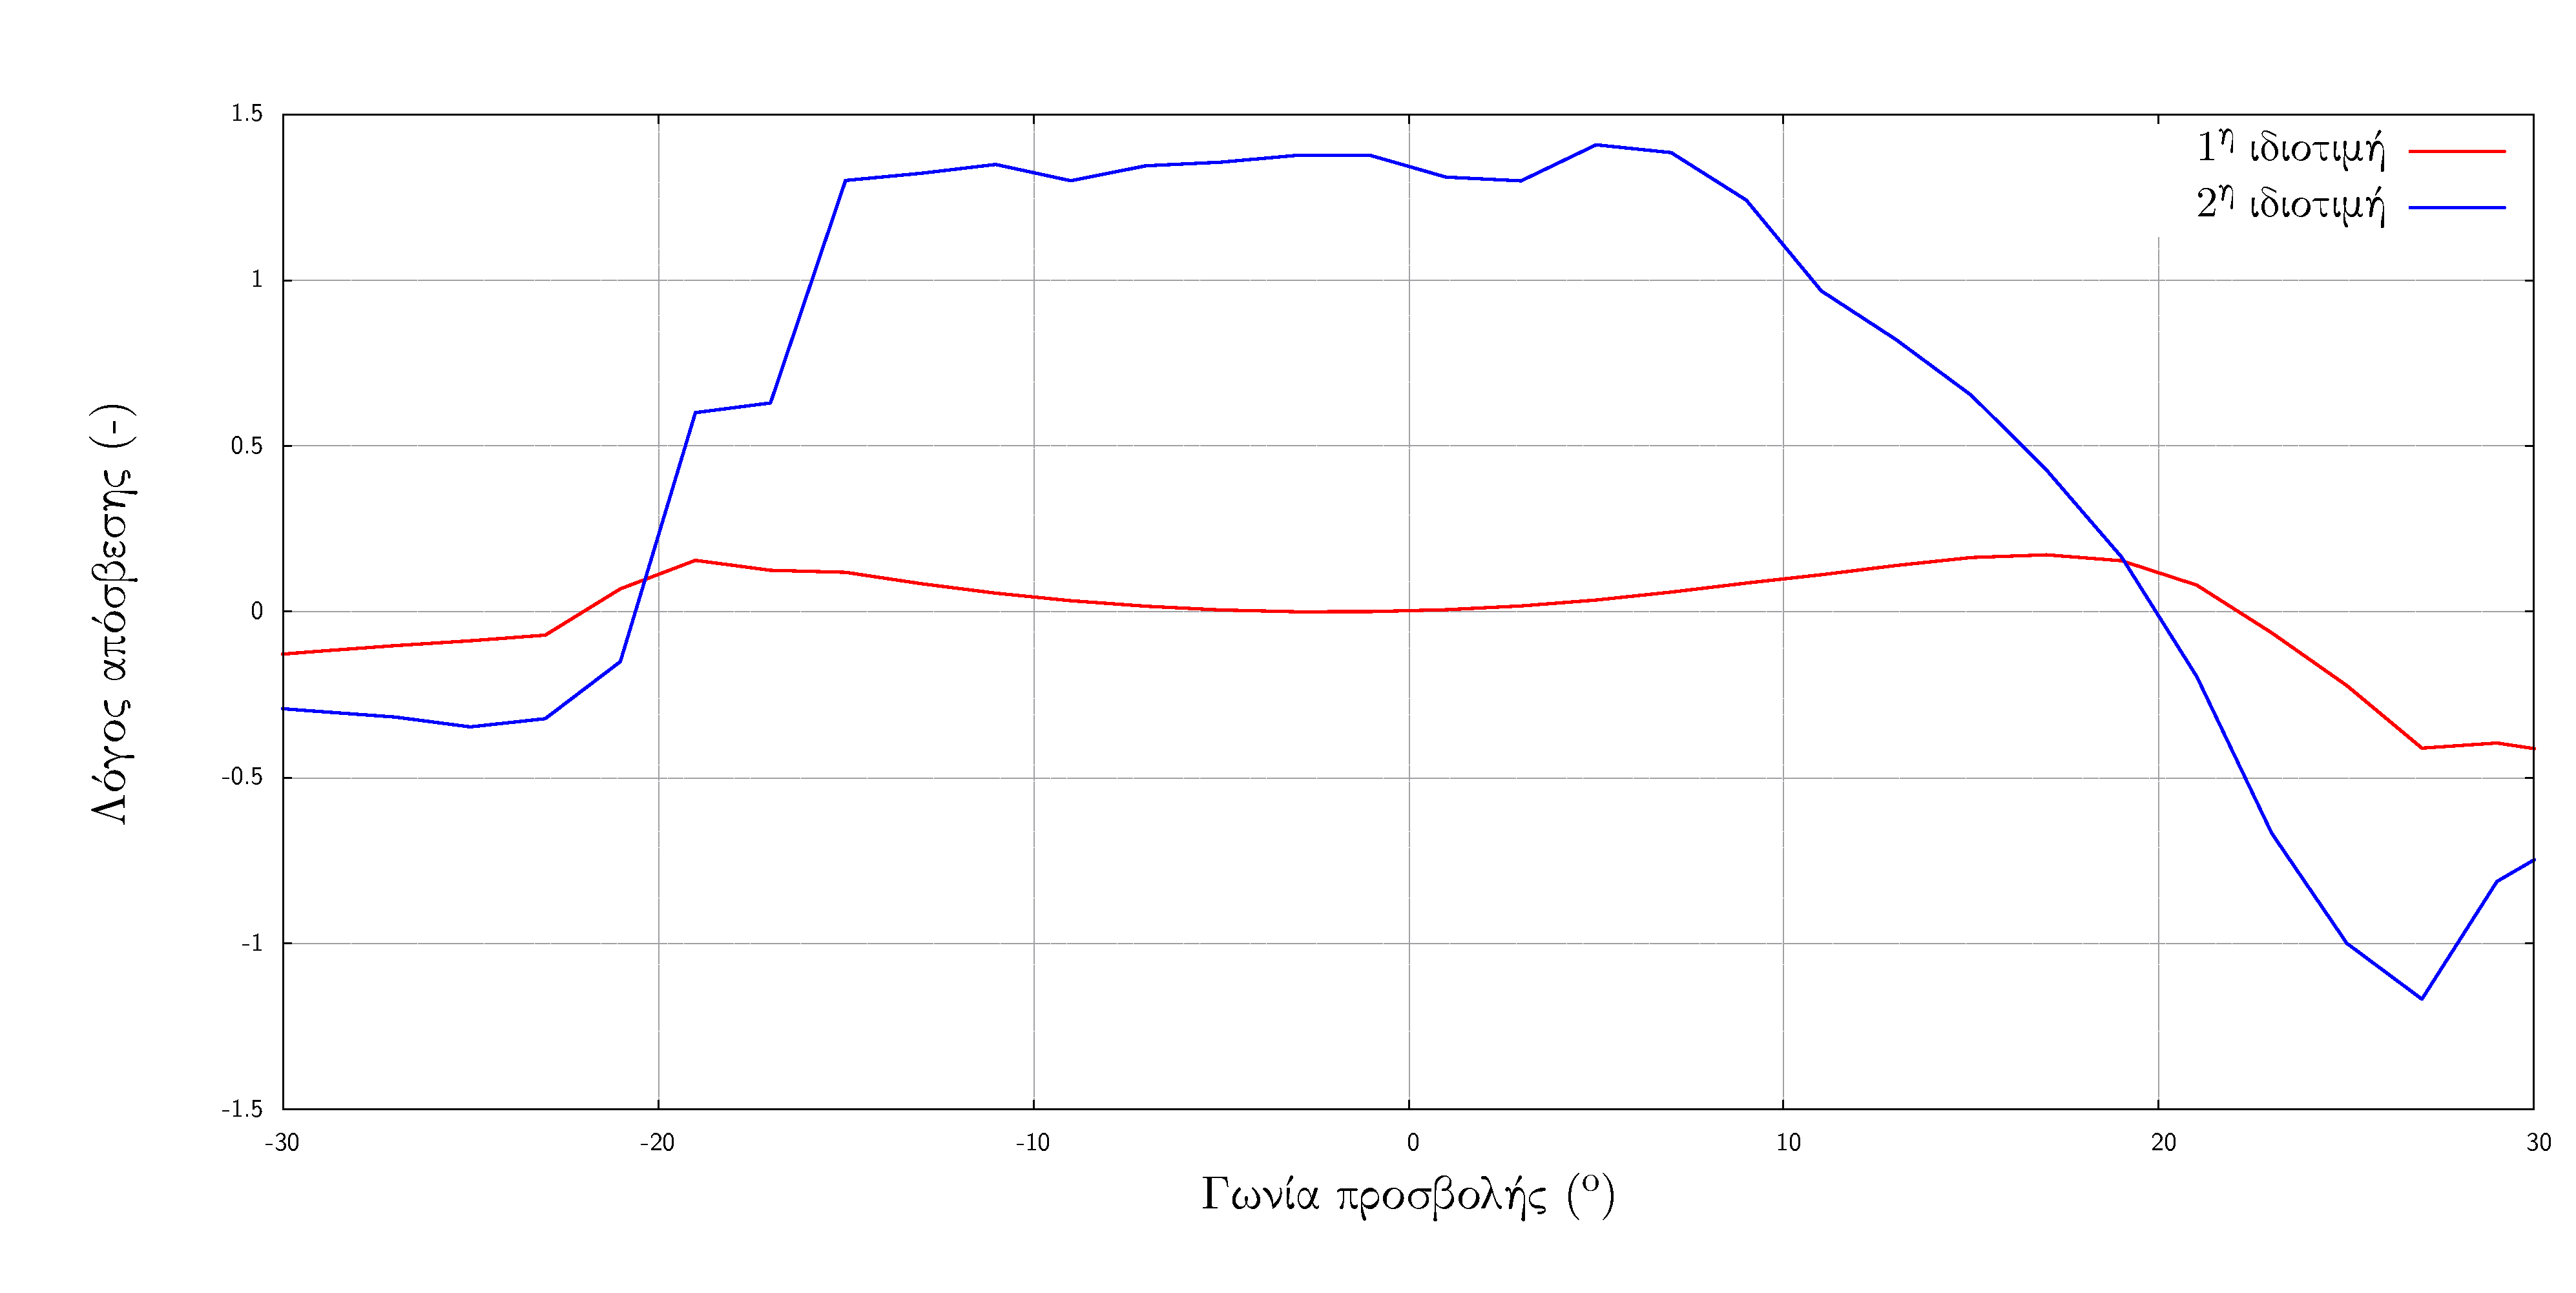
\includegraphics[width=0.95\textwidth]{./figures/aoa_vs_damp.pdf}
    \end{center}
    \caption{Μεταβολή του λόγου απόσβεσης συναρτήσει της γωνίας προσβολής}
    \label{fig:damping}
\end{figure}

\begin{figure}
    \begin{center}
        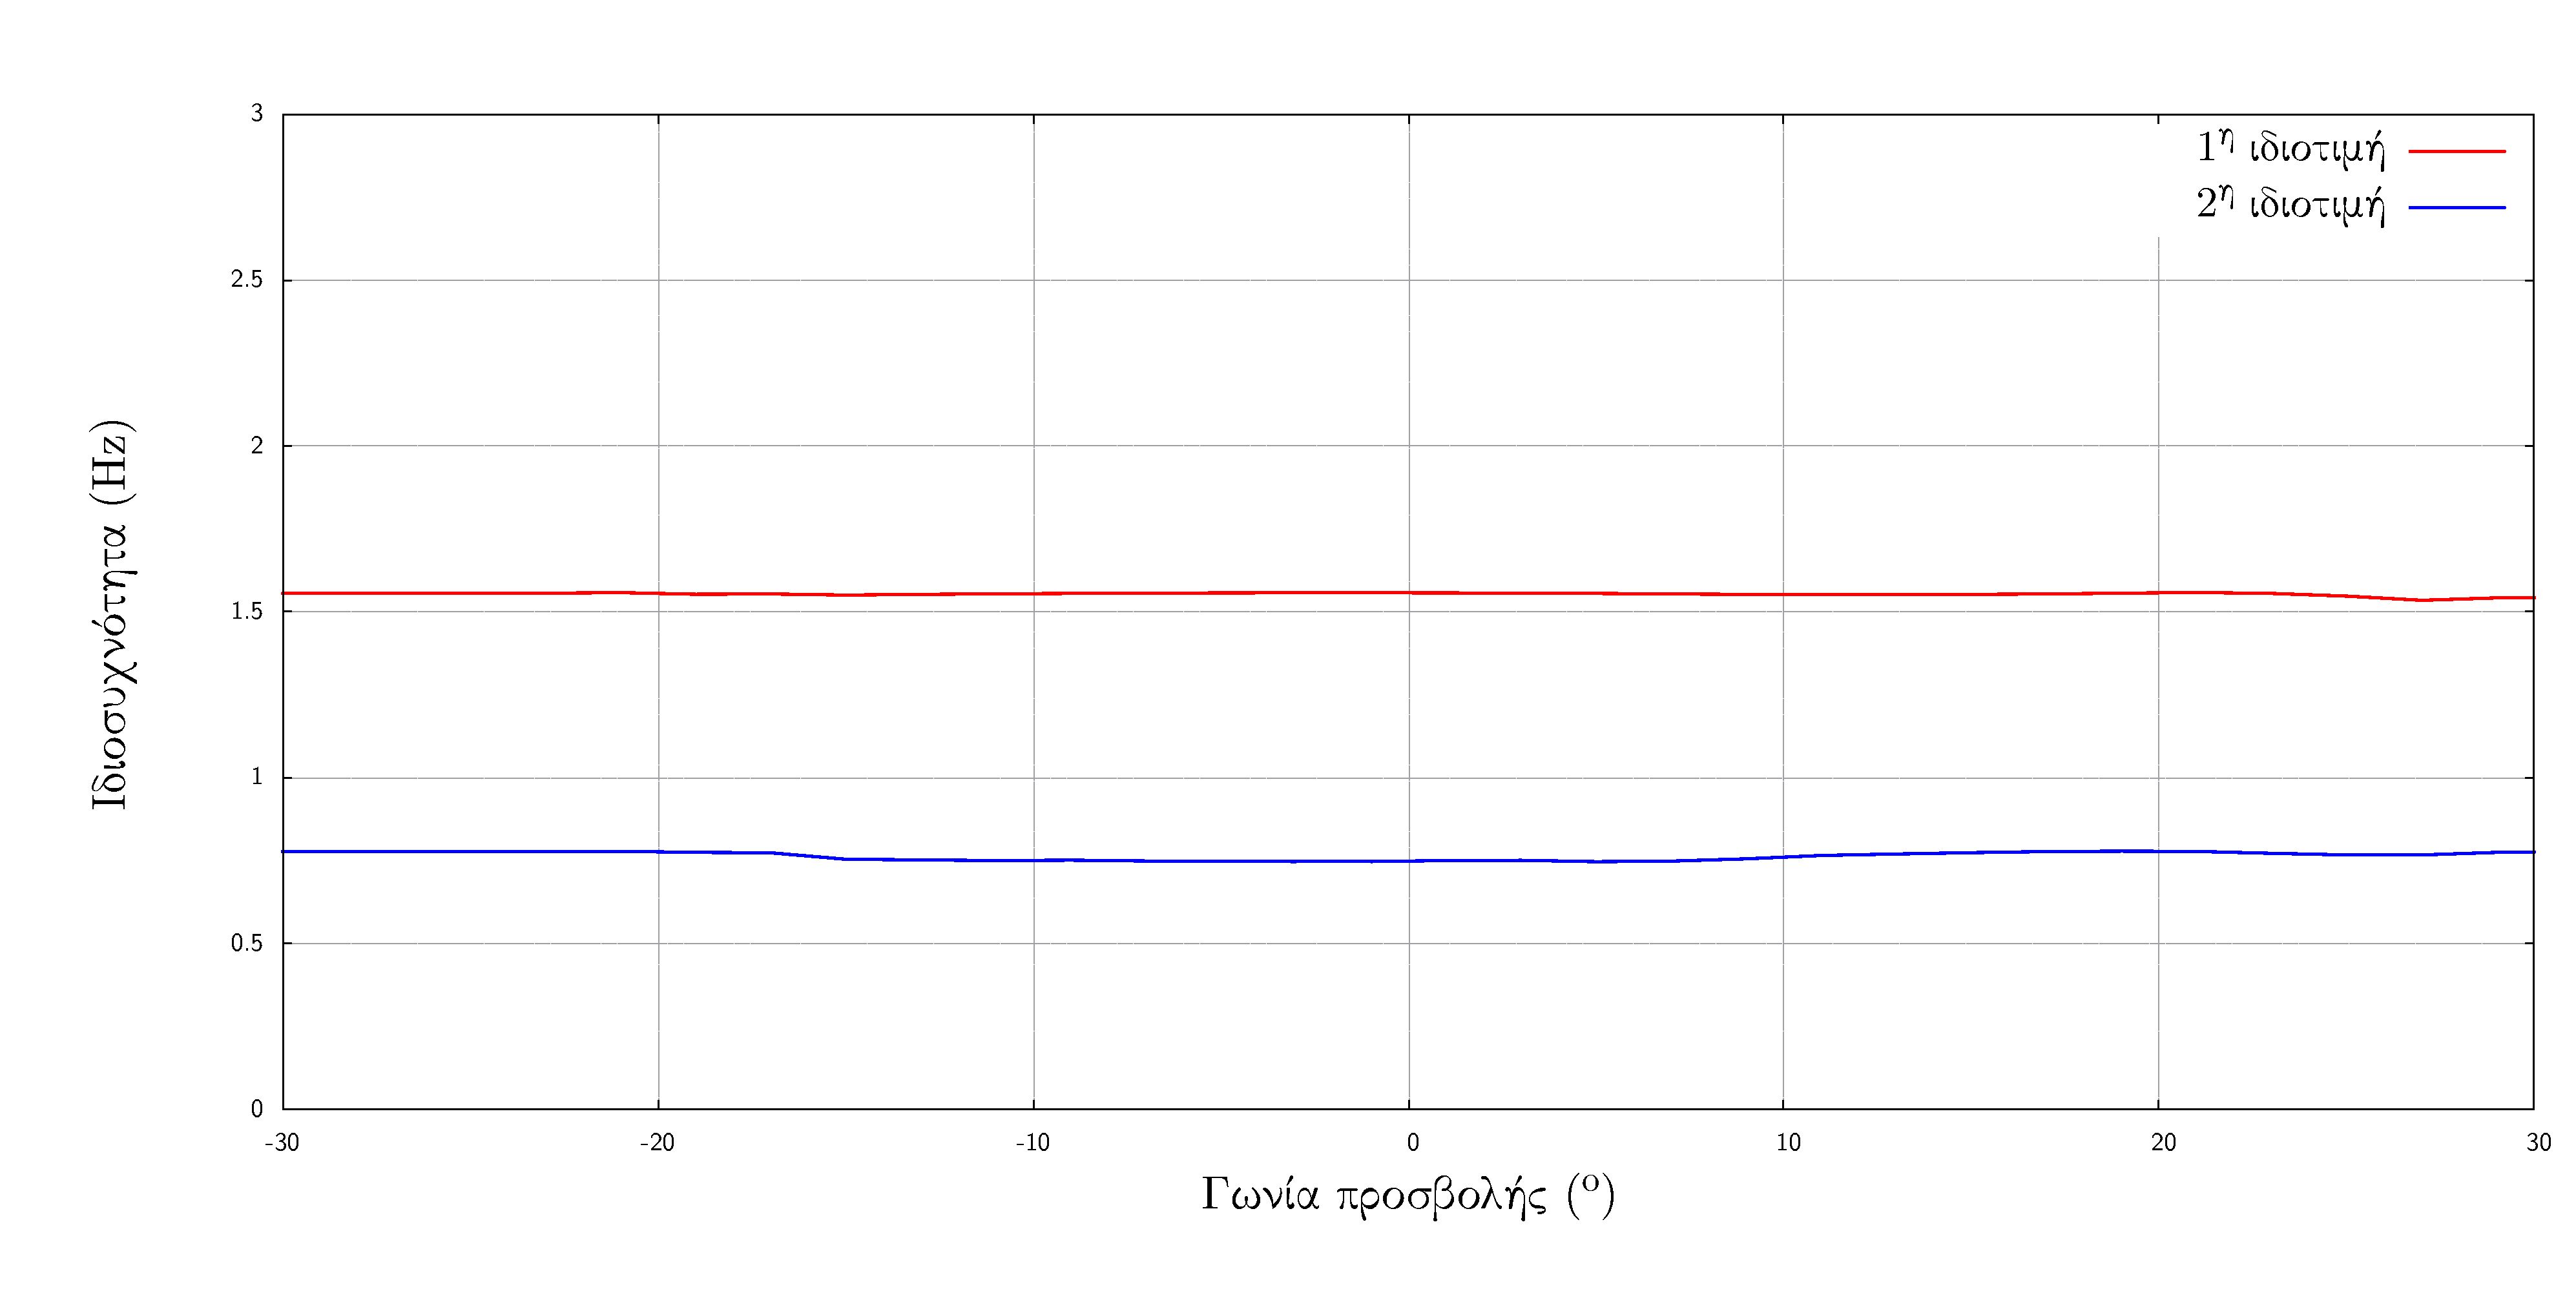
\includegraphics[width=0.95\textwidth]{./figures/aoa_vs_freq.pdf}
    \end{center}
    \caption{Μεταβολή των ιδιοσυχνοτήτων συναρτήσει της γωνίας προσβολής}
    \label{fig:frequency}
\end{figure}

Η απόσβεση του συστήματος γίνεται αρνητική, δηλαδή το σύστημα γίνεται ασταθές, όταν ένας εκ των δύο λόγους απόσβεσης γίνει αρνητικός, διότι αυτό υποδηλώνει πως προσδίδεται ενέργεια στην αεροτομή απο το ρευστό. Στο σχήμα \ref{fig:damping}, όπως υποδηλώνει και η \cref{eq:eigenvalue} βλέπουμε το πραγματικό μέρος της ιδιοτιμής και φαίνεται να γίνεται αρνητικό για γωνία προσβολής περίπου $20^o$ και $\approx-21^o$ όταν η ιδιοτιμή που αντιστοιχεί στον Β.Ε πτερύγησης γίνεται αρνητική. Παρατηρούμε επίσης, πως το μεγαλύτερο μέρος της απόσβεσης παρέχεται απο τον Β.Ε πτερύγησης (flapwise) , ενώ για την chordwise κίνηση έχουμε μικρές αλλά θετικές τιμές απόσβεσης. Τέλος, παρατηρούμε πως οι ιδιοσυχνότητες επηρεάζονται ελάχιστα απο τη γωνία προσβολής.

Για τα δεδομένα του προβλήματος μας (πίνακας \ref{tab:data}) οι δυο ιδιοσυχνότητες και λόγοι απόσβεσης φαίνονται στον πίνακα \ref{tab:res}.

\begin{table}[ht!]
    \begin{center}
        \begin{tabular}[c]{|r|c|c|}
            \hline
            ~ & $1^{\text{η}}$ ιδιοτιμή & $2^{\text{η}}$ ιδιοτιμή\\
            \hline
            Ιδιοσυχνότητα (Hz) & 1.55 & 0.75 \\
            Λόγος απόσβεσης (--) & 0.037 & 1.325 \\
            \hline
        \end{tabular}
    \caption{Ιδιοτιμές συστήματος}
    \label{tab:res}
    \end{center}
\end{table}


Τα ιδιοδιανύσματα που προκύπτουν απο την ανάλυση οπτικοποιούνται στο σχήμα \ref{fig:eigenvectors}. Ο βρόγχος που σχηματίζεται υποδηλώνει την παρουσία απόσβεσης, και υπεισέρχεται ως διαφορά φάσης μεταξύ των ταλαντώσεων με τις δυο ιδιοσυχνότητες. Όπως είναι φανερό και απο τον πίνακα \ref{fig:res} η πρώτη ιδιομορφή εμφανίζει πολύ μικρότερο βρόγχο που συμφωνεί με τον μικρότερο λόγο απόσβεσης της ιδιοτιμής.

\begin{figure}[ht!]
    \begin{center}
        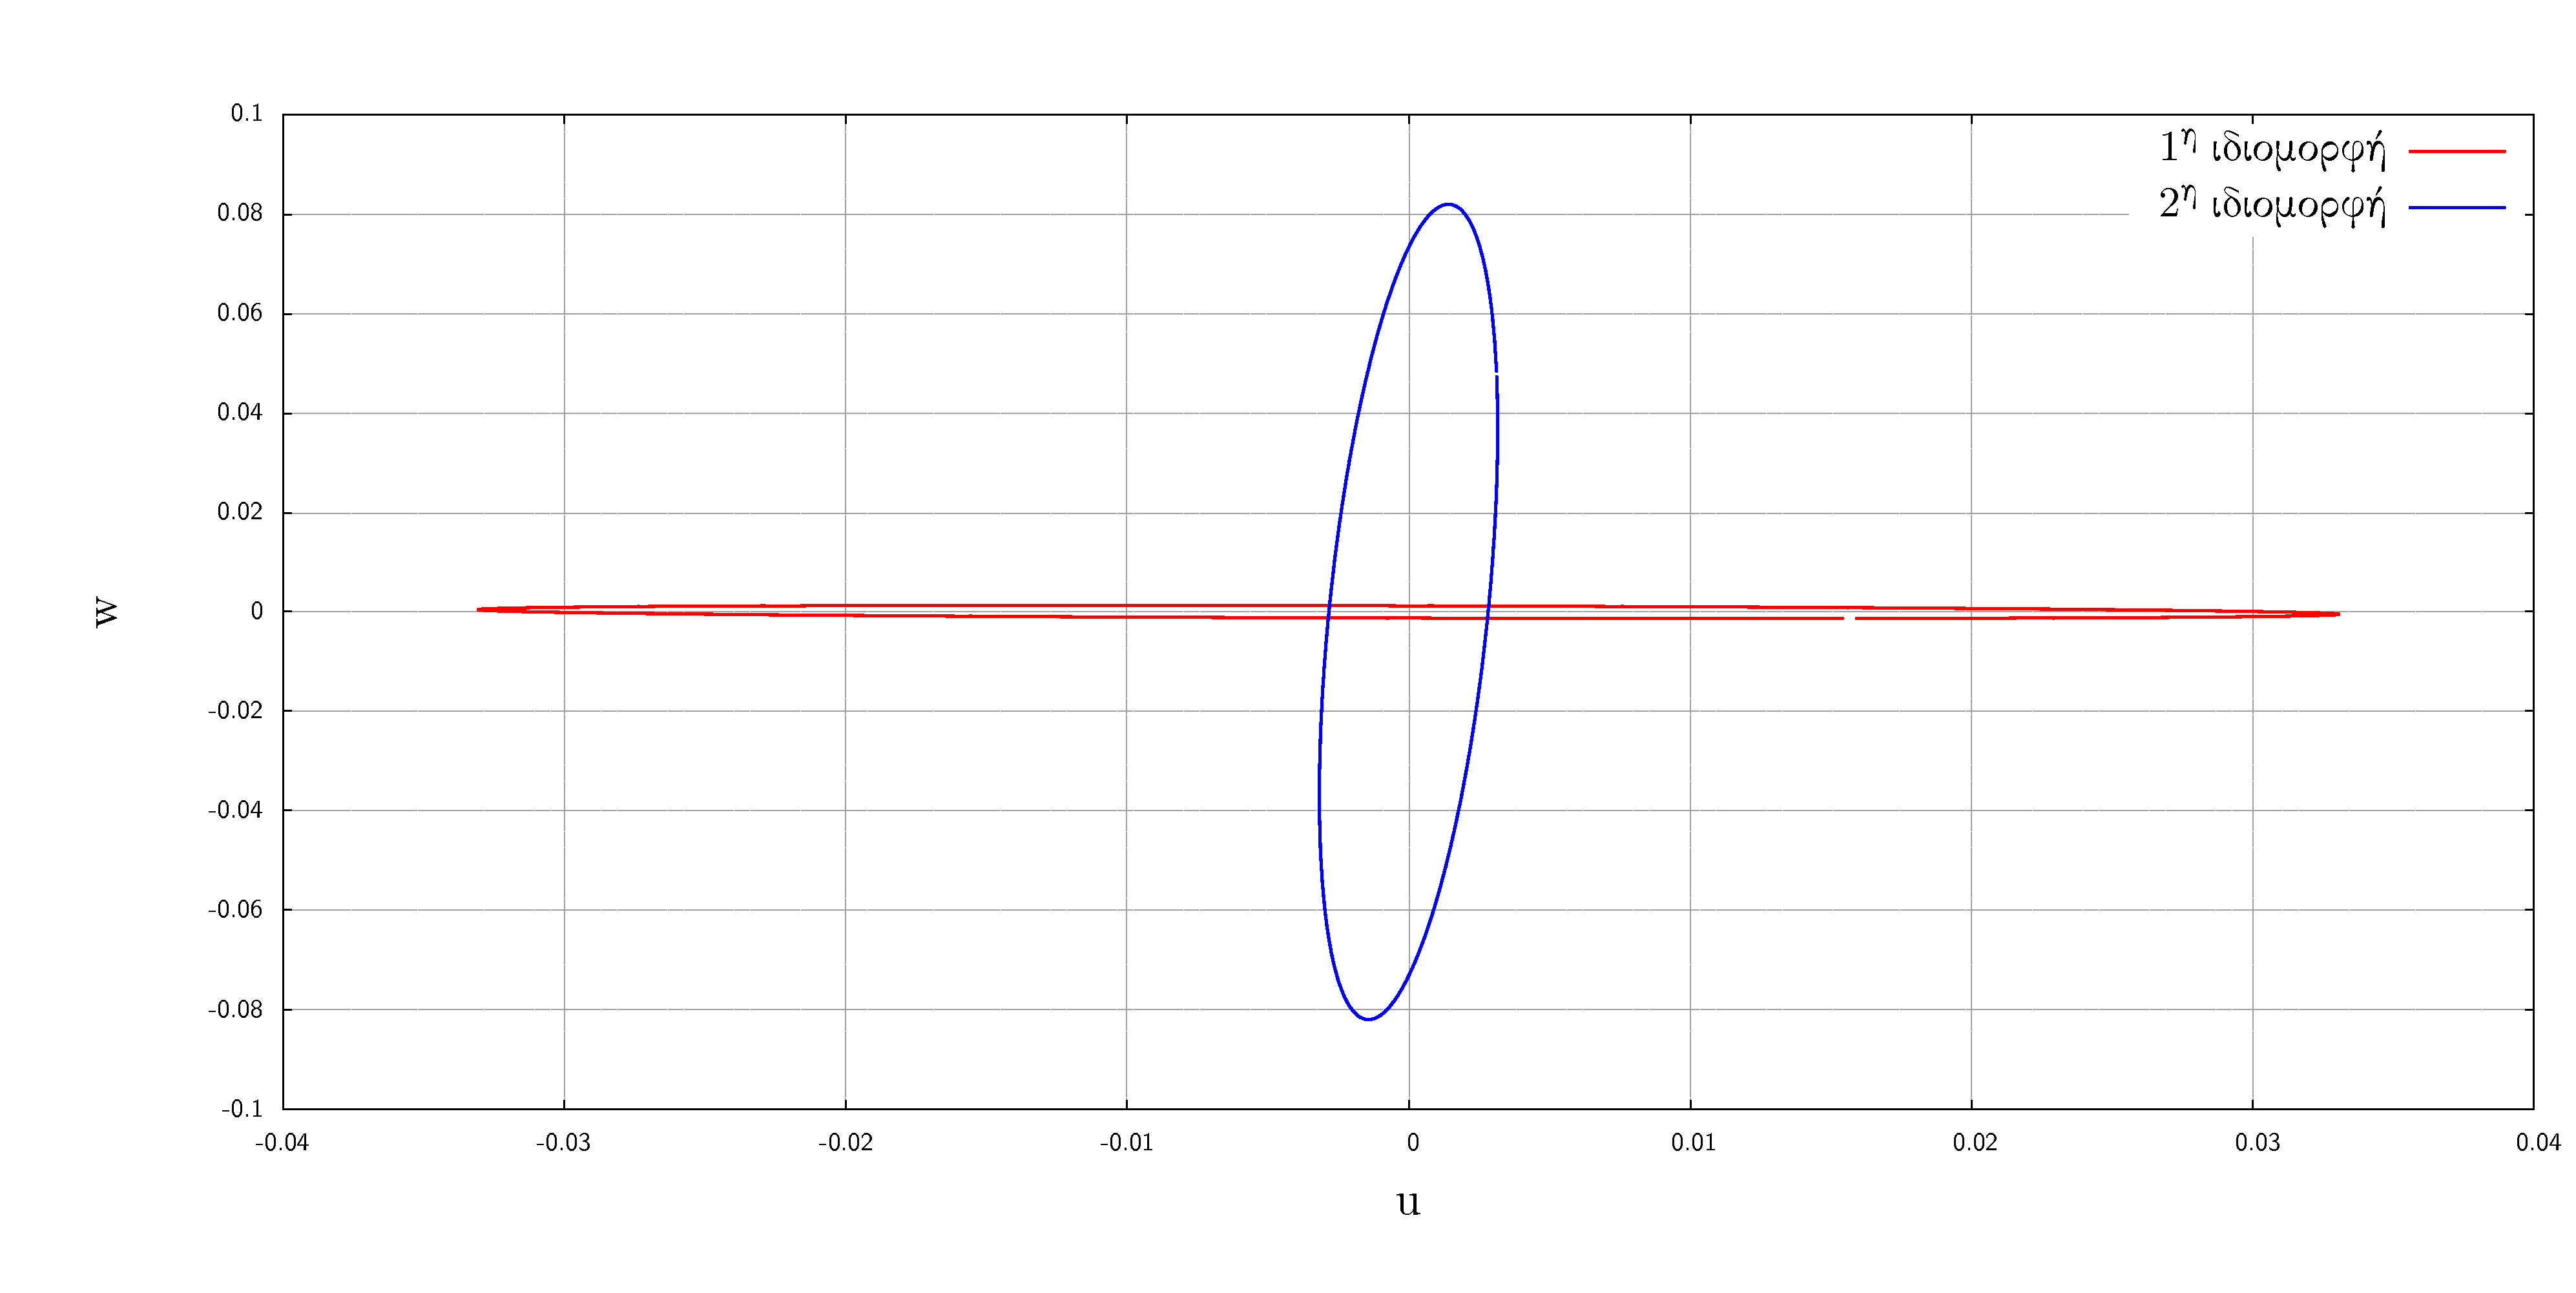
\includegraphics[width=0.95\textwidth]{./figures/eigenvectors.pdf}
    \end{center}
    \caption{Οπτικοποίηση ιδιοδιανυσμάτων για τις δυο ιδιοτιμές}
    \label{fig:eigenvectors}
\end{figure}
